\chapter{Reflex Enterprise Stack: Implementation Architecture}

\section{Four-Layer Stack Architecture}

The Reflex Enterprise stack implements the Chatman Equation through four integrated layers:

\begin{equation}
\text{Reflex} = (\text{unrdf}, \text{KNHK}, \text{ggen}, \text{Lockchain})
\end{equation}

Each layer addresses one aspect of the measurement function \(\measure(\obs) = A\):

\begin{center}
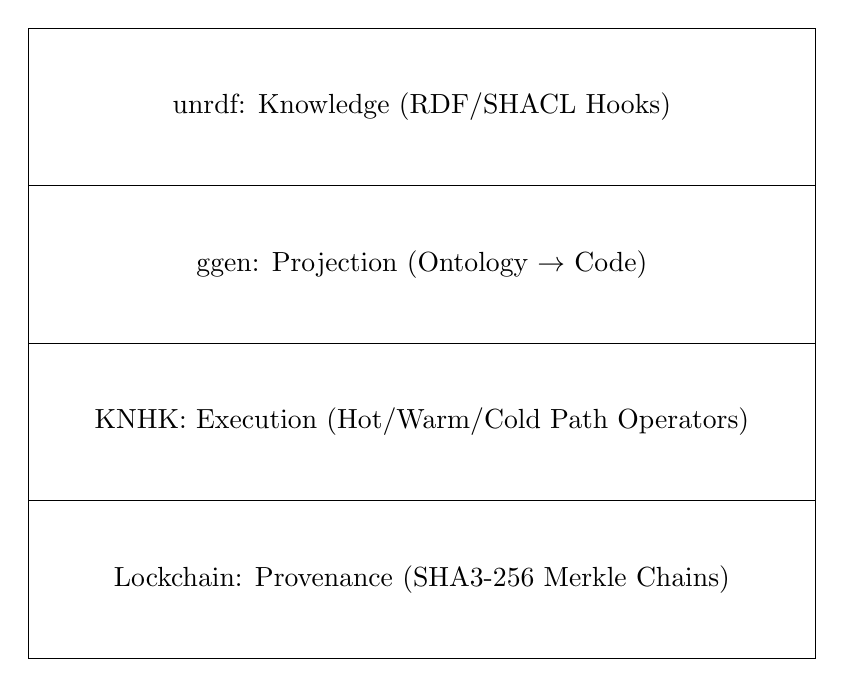
\begin{tikzpicture}
  \draw (0, 0) rectangle (10, 2) node[pos=.5] {Lockchain: Provenance (SHA3-256 Merkle Chains)};
  \draw (0, 2) rectangle (10, 4) node[pos=.5] {KNHK: Execution (Hot/Warm/Cold Path Operators)};
  \draw (0, 4) rectangle (10, 6) node[pos=.5] {ggen: Projection (Ontology \(\to\) Code)};
  \draw (0, 6) rectangle (10, 8) node[pos=.5] {unrdf: Knowledge (RDF/SHACL Hooks)};
\end{tikzpicture}
\end{center}

\section{Layer 1: unrdf — Knowledge Hooks}

\textbf{Role}: Provides the bounded autonomic layer of Reflex. Knowledge Hooks detect, validate,
and enforce enterprise rules via RDF and SHACL.

\textbf{Responsibilities}:

\begin{enumerate}
  \item \textbf{Change Detection}: Monitor RDF knowledge graph for triggering events
  \item \textbf{Constraint Validation}: Enforce SHACL shape constraints at ingress
  \item \textbf{Rule Evaluation}: Execute SPARQL ASK queries for guard conditions
  \item \textbf{Observability}: Emit OpenTelemetry spans for each hook execution
  \item \textbf{Receipt Generation}: Produce Merkle-linked proof of execution
\end{enumerate}

\textbf{Components}:

\begin{lstlisting}[language=Rust]
pub mod unrdf {
    /// RDF knowledge graph representation
    pub struct RdfGraph {
        triples: HashSet<Triple>,
        schema: Option<ShapeSchema>,
    }

    /// Knowledge hook implementation
    pub struct KnowledgeHook {
        trigger: SparqlQuery,
        check: ShaplConstraint,
        act: WorkflowPattern,
    }

    /// Hook execution engine
    pub struct HookEngine {
        hooks: Vec<KnowledgeHook>,
        graph: RdfGraph,
    }

    impl HookEngine {
        pub fn evaluate(&self, delta: &RdfGraph) -> Result<HookResult, Error> {
            // 1. Trigger detection
            // 2. Constraint validation (SHACL)
            // 3. Guard checking
            // 4. Action routing to KNHK
            // 5. Receipt generation
        }
    }
}
\end{lstlisting}

\textbf{SLO}: Warm path \(\leq 500\) ms for hook service time (P99).

\section{Layer 2: KNHK — Execution Engine}

\textbf{Role}: Implements the measurement operator \(\measure(\obs)\) in three performance tiers.

\textbf{Characteristics}:

\begin{enumerate}
  \item \textbf{Hot Path (C)}: \(\leq 8\) ticks (\(\leq 2\) ns) for rule checks (ASK, COUNT, COMPARE, VALIDATE)
  \item \textbf{Warm Path (Rust)}: \(\leq 500\) ms for workflow orchestration and ETL
  \item \textbf{Cold Path (Erlang/SPARQL)}: \(\leq 500\) ms for complex queries and reasoning
\end{enumerate}

\textbf{Operators}: All 43 YAWL patterns implemented as deterministic operators with guard
enforcement and receipt generation.

\begin{lstlisting}[language=Rust]
pub mod knhk {
    /// Operator trait: all patterns implement this
    pub trait WorkflowOperator {
        fn execute(&self, obs: &RdfGraph) -> Result<Action, Error>;
        fn get_slo(&self) -> SLOBound;
        fn get_pattern_id(&self) -> u32;
    }

    /// Hot path operator
    pub struct HotPathOperator {
        pattern_id: u32,
        logic: fn(&RdfGraph) -> Action,
    }

    /// Warm path operator
    pub struct WarmPathOperator {
        pattern_id: u32,
        orchestration: Arc<dyn Fn(&RdfGraph) -> Action + Send + Sync>,
    }

    /// Guard enforcement
    pub struct GuardCheckerFactory {
        legality: Box<dyn Fn(&Action) -> bool>,
        budget: Box<dyn Fn(&Action) -> bool>,
        chronology: Box<dyn Fn(&Action) -> bool>,
        causality: Box<dyn Fn(&Action) -> bool>,
    }
}
\end{lstlisting}

\textbf{Key Property}: Every operator is deterministic, type-safe, and produces a receipt.

\textbf{SLO}:
\begin{itemize}
  \item Hot path \(\leq 2\) ns (P99)
  \item Warm path \(\leq 500\) ms (P99)
  \item Cold path \(\leq 500\) ms (P99)
\end{itemize}

\section{Layer 3: ggen — Code Projection}

\textbf{Role}: Operationalizes bounded regeneration. Reprojects ontology schemas into code
across multiple languages until no measurable drift exists.

\textbf{Workflow}:

\begin{equation}
\text{RDF Ontology} \xrightarrow{\text{ggen}} \text{Rust Code} \xrightarrow{\text{compile}} \text{Deterministic Operators}
\end{equation}

\begin{equation}
\text{RDF Ontology} \xrightarrow{\text{ggen}} \text{TypeScript Code} \xrightarrow{\text{transpile}} \text{JavaScript Targets}
\end{equation}

\begin{lstlisting}[language=Rust]
pub mod ggen {
    /// Ontology compiler
    pub struct OntologyCompiler {
        ontology: RdfGraph,
        schema: ShapeSchema,
    }

    /// Code generation context
    pub struct CodeGenContext {
        target_languages: Vec<Language>,
        max_iterations: u32,
        drift_tolerance: f64,  // 0.5%
    }

    impl OntologyCompiler {
        pub fn regenerate(
            &mut self,
            context: &CodeGenContext,
        ) -> Result<RegenerationResult, Error> {
            let mut iteration = 0;
            let mut current_drift = 1.0;

            while current_drift > context.drift_tolerance
                && iteration < context.max_iterations
            {
                // 1. Generate code from ontology
                let generated = self.generate_code()?;

                // 2. Compile generated code
                let compiled = self.compile(&generated)?;

                // 3. Measure drift
                current_drift = self.measure_drift(&compiled)?;

                // 4. Emit receipt
                let receipt = Receipt::regeneration(current_drift);

                iteration += 1;
            }

            Ok(RegenerationResult {
                iterations: iteration,
                final_drift: current_drift,
                receipt,
            })
        }
    }
}
\end{lstlisting}

\textbf{Key Property}: Regeneration halts when drift \(\leq 0.5\%\) or receipt delta \(<10^{-3}\).

\textbf{SLO}: Regeneration halts when \(\drift(\Sigma) \leq \epsilon\) (typically 0.5\%).

\section{Layer 4: Lockchain — Provenance Layer}

\textbf{Role}: Provides SHA3-256 Merkle chains for all actions. Replays must reproduce
\(h(A) = h(\measure(\obs))\) within tolerance.

\textbf{Receipt Components}:

\begin{lstlisting}[language=Rust]
pub mod lockchain {
    /// Merkle-linked receipt
    #[derive(Debug, Clone, Serialize, Deserialize)]
    pub struct Receipt {
        // Hashes of execution context
        pub h_obs: [u8; 32],          // SHA3-256(observations)
        pub h_gamma: [u8; 32],        // SHA3-256(candidates)
        pub h_guards: [u8; 32],       // SHA3-256(guard_set)
        pub h_action: [u8; 32],       // SHA3-256(action)
        pub h_measure: [u8; 32],      // SHA3-256(measure function)

        // Merkle chain link
        pub merkle_root: [u8; 32],    // SHA3-256(receipt | prev_merkle)
        pub prev_merkle: [u8; 32],    // Previous receipt's merkle_root

        // Metadata
        pub timestamp: u64,
        pub actor: String,
        pub slo: String,
    }

    impl Receipt {
        pub fn verify(&self, obs: &RdfGraph, action: &Action) -> bool {
            // Recompute hashes
            let computed_h_obs = sha3_256(obs);
            let computed_h_action = sha3_256(action);

            // Verify chain
            computed_h_obs == self.h_obs
                && computed_h_action == self.h_action
                && self.merkle_root == sha3_256((self, self.prev_merkle))
        }

        pub fn compute_merkle_root(&self) -> [u8; 32] {
            sha3_256((self, self.prev_merkle))
        }
    }

    /// Immutable audit log
    pub struct AuditLog {
        receipts: Vec<Receipt>,
    }

    impl AuditLog {
        pub fn append(&mut self, receipt: Receipt) -> Result<(), Error> {
            // Verify receipt chain against previous
            if let Some(last) = self.receipts.last() {
                receipt.prev_merkle == last.merkle_root
            } else {
                true
            }?;

            self.receipts.push(receipt);
            Ok(())
        }

        pub fn verify_all(&self) -> bool {
            for i in 1..self.receipts.len() {
                if self.receipts[i].prev_merkle
                    != self.receipts[i - 1].merkle_root
                {
                    return false;
                }
            }
            true
        }
    }
}
\end{lstlisting}

\textbf{Key Property}: Every receipt cryptographically links to the previous one, creating
an immutable, tamper-evident chain.

\textbf{SLO}: Receipt delta \(<10^{-3}\) within tolerance.

\section{Stack Integration Flow}

The four layers operate in a closed-loop cycle:

\begin{enumerate}
  \item \textbf{Ingress}: Change \(\Delta \obs\) detected in knowledge graph
  \item \textbf{unrdf}: Hook evaluation detects trigger, validates constraints, routes to pattern
  \item \textbf{KNHK}: Operator executes pattern, enforces guards, produces action
  \item \textbf{ggen}: If schema changed, regenerate ontology projection (iteratively)
  \item \textbf{Lockchain}: Append receipt to immutable audit log
  \item \textbf{Verification}: Independent recomputation validates \(h(A) = h(\measure(\obs))\)
\end{enumerate}

\begin{equation}
\Delta \obs \xrightarrow{\text{unrdf}} \text{trigger} \xrightarrow{\text{KNHK}} A
  \xrightarrow{\text{ggen}} \text{regen} \xrightarrow{\text{Lockchain}} \receipt
\end{equation}

\section{Stack Economics}

\subsection{Cost Model}

\begin{table}[H]
\centering
\caption{Stack Cost Breakdown}
\begin{tabular}{|l|l|l|}
\hline
\textbf{Layer} & \textbf{Cost Component} & \textbf{Amortized Cost} \\
\hline
unrdf & SPARQL query evaluation, SHACL validation & 0.01--0.1 cent \\
\hline
KNHK & Hot path (\(\leq 8\) ticks) + receipt & Micro-cent \\
\hline
ggen & Regeneration (amortized per decision) & Negligible \\
\hline
Lockchain & Receipt write and verification & Negligible \\
\hline
\end{tabular}
\end{table}

Total cost per decision: \(\leq 0.1\) cent on average.

\subsection{Throughput Model}

\begin{equation}
\text{Throughput} = \frac{\text{# Hooks} \times \text{Average Triggers per Hook}}{\text{SLO Bound}}
\end{equation}

Example:
\begin{itemize}
  \item 1,000 hooks
  \item Average 0.1 triggers per hook per second
  \item SLO: 2 ns (hot path)
  \item Throughput: \(\frac{1000 \times 0.1}{2 \times 10^{-9}} = 50\) billion decisions per second
\end{itemize}

Throughput is independent of headcount. Scaling requires adding hooks, not workers.

\section{Non-Functional Properties}

\begin{table}[H]
\centering
\caption{Stack Non-Functional Properties}
\begin{tabular}{|l|l|l|}
\hline
\textbf{Property} & \textbf{Mechanism} & \textbf{Guarantee} \\
\hline
Determinism & Pure functions, no side effects & 100\% \\
\hline
Availability & Distributed hook execution & 99.99\% \\
\hline
Consistency & Guard enforcement before action & Strong \\
\hline
Latency & Three-tier SLO architecture & \(\leq 2\) ns (hot) \\
\hline
Auditability & Cryptographic receipt chain & Bit-perfect reproducibility \\
\hline
Recoverability & Immutable audit log & Full replay capability \\
\hline
Compliance & Guard-based control mapping & SOX/HIPAA/PCI alignment \\
\hline
\end{tabular}
\end{table}
